\newpage
\section{顾客端AI功能}
\label{sec:guest_features}

\begin{figure}[htbp]
	\centering
	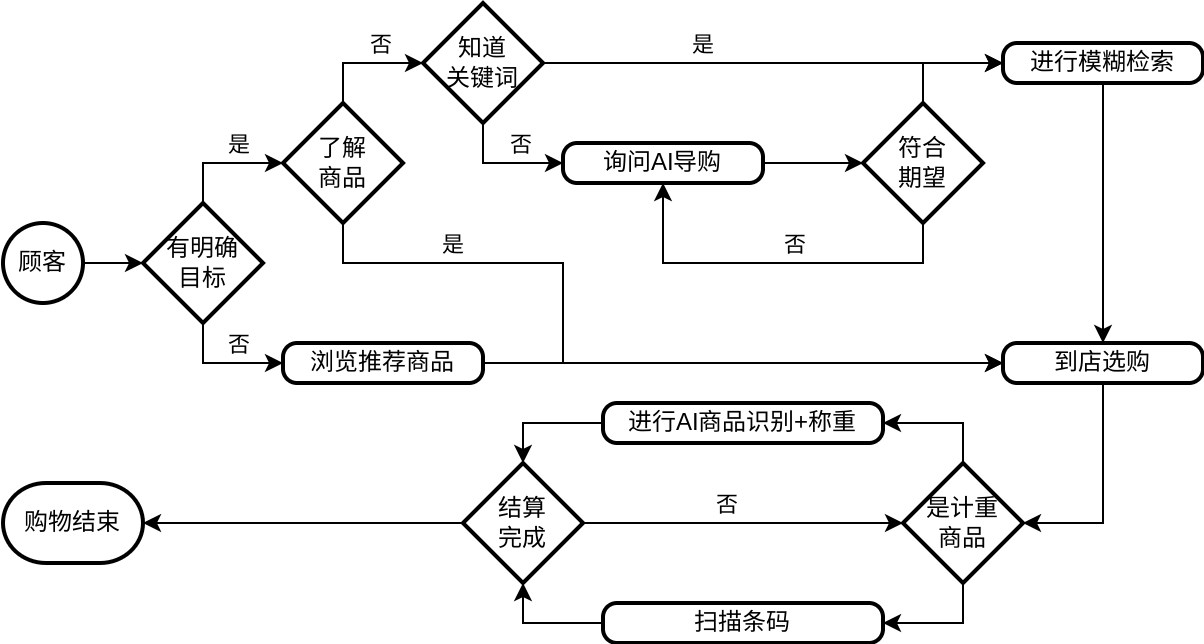
\includegraphics[width=0.8\textwidth]{./imgs/choose-n-buy.png}
	\caption{最终消费者商品选购流程}
	\label{fig:choose-n-buy}
\end{figure}

面向最终消费者的AI功能主要围绕着发现心仪商品和结算所购买商品的场景(如图 \ref{fig:choose-n-buy} 所示)展开。顾客发现商品的方式大致可以分为目的导向的和非目的导向的商品发现方式,其中非目的导向的商品发现方式与商户的宣传手段及其有效性关联较大,很大程度上取决于顾客是否浏览到该商铺对应宣传内容(实体、在线广告、客户群等)和对于宣传内容的实际吸引力。宣传内容的曝光可以由从业人员对社交媒体的参与来实现,而宣传内容可以借助上一部分提及的AI商品文案起草特性来辅助。目的导向的发现方式更为复杂。

目的导向的商品发现方式主要包括用户对商品进行搜索的过程。对于叫法比较单一、名称好记没有歧义的商品,简单分词---匹配的关键词搜索功能是可以满足需要的。然而,时间情况下商品名称匹配的问题可能远复杂于理想的情况。例如笼统和详细说法的区别:“可乐”和“苏打水”都可以叫作“汽水”,但这三个词语之间却无法直接相互匹配,并且若是为此将“汽水”拆为“汽”和“水”,不但仍然无法和“可乐”匹配,还可能会误匹配到与如“水”、“水汽”等词语相关的其他商品。

为了在一定程度上解决该问题,本设计包含模糊搜索引擎项目“探寻”及其对应词典处理脚本。该子项目采用“结巴”分词库\cite{sun_fxsjyjieba_2025,messense_messensejieba-rs_2025}进行分词,并且利用大语言模型对每个词语的近义词进行枚举,最后将各个来源的处理结果整理为高查询效率的格式在为中文优化的自定义搜索算法中进行部署,以此在消耗比较少的计算资源的情况下达到较高的搜索速度和(中文)搜索的准确率,有助于最终消费者更好地进行目的导向的商品发现活动,推动消费体验、营业质量提升。

然而性能更加强大的模糊搜索系统无法解决在许多情况下顾客不知悉需要搜索的关键词(及其近义词)的问题,这种情况下,顾客可能甚至并不清楚自己实际需要的商品。这个问题较为明显的解决思想是使得“商品发现”相关功能具有理解消费者对其需求的描述的语义并将需求内容对应于特定商品信息,或者为此生成对应的搜索语句提供给用户进行检索(或自动运行检索)。

为了解决这种情况带来的问题,该设计的顾客端移动应用程序包含AI导购助手模块。该模块利用经过特定提示词引导的多轮LLM对话及单次LLM调用,分别营造与顾客进行导购交流、导购向用户提出购买建议,如此往复的体验;从导购对用户的回复中提取出适用于检索的关键词语句,以此实现消费者只要合理形容需求,便可检索到对应商品的功能。

AI识别计重商品结算模块是该设计对一般传统实体零售流程的另一个改进。通过利用AI物体识别算法,在零售管理系统中整合物体识别AI模型的训练数据采集、标注等操作对应的用户界面,自动化模型训练和部署的过程;在结算终端中整合AI物体识别前端软件及摄像头、质量传感器等硬件来实现营业者轻松部署AI物体识别模型,最终用户轻松自助结算计重商品,去除计重商品结算过程对店员参与的要求。

\subsection{导购助手}

\begin{figure}[htbp]
	\centering
	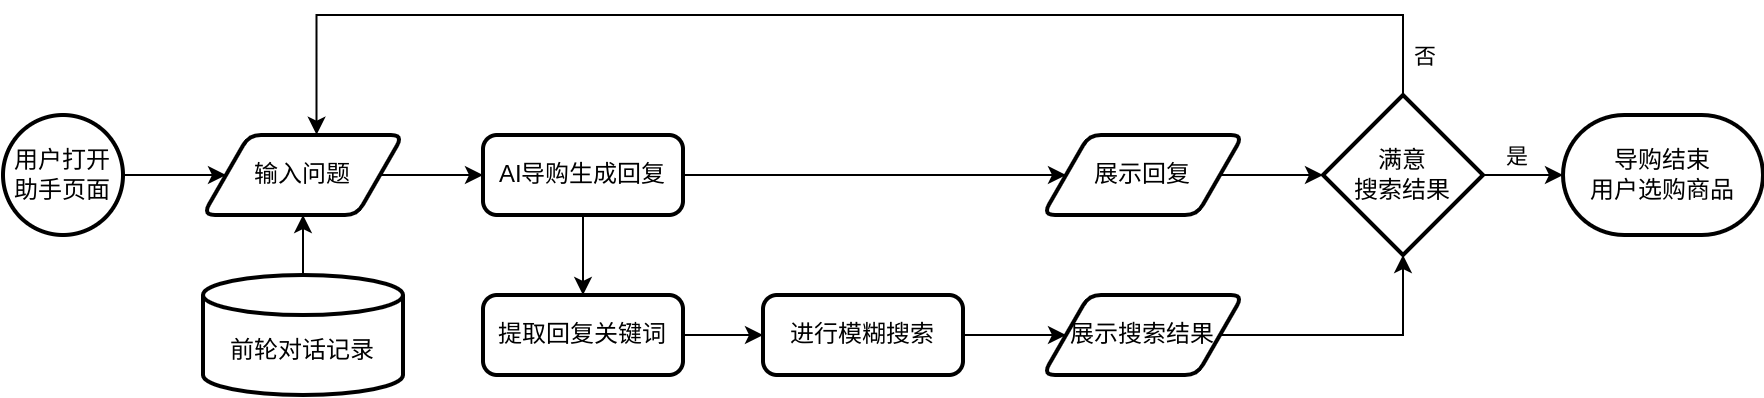
\includegraphics[width=0.8\textwidth]{./imgs/ask-n-choose.png}
	\caption{最终消费者导购操作流程}
	\label{fig:ask-n-choose}
\end{figure}

导购助手工作流程如图 \ref{fig:ask-n-choose} 所示,主要包括以下两个部分:

\begin{itemize}
    \item \textbf{对话式AI导购专家:} 通过与最终消费者的一轮或多轮对话确定消费者的具体需求,并给出相应的购买建议(商品类型、名称等)。
    \item \textbf{搜索关键词猜测算法:} 通过利用大语言模型强大的文字处理能力,使用AI导购的输出产生出对应的搜索关键词。
\end{itemize}

\subsubsection{对话型生成式AI}

AI导购专家实质上就是扮演导购身份,可以与用户进行多轮对话,解决用户困扰的人工智能聊天机器人(chatbot)。为了使得输出较为中性的无(行业相关)微调的一般大语言模型输出符合“导购身份”的回复,而不是一般的建议,该设计开发了以下的系统、对话提示模板:

\begin{itemize}
    \item[] \textbf{系统:}You are a helpful assistant of a retail shop that advise about buying stuffs.\footnote{此处为开发方便(并且遵照“百炼”官方文档中系统提示的风格)使用了英文系统提示,但实际测试中AI发挥了语言中性的能力,正确地使用中文响应了中文编写的输入。若需要中文提示,可以使用:你是零售商店的一个乐于助人的导购,你向客人提出购物建议。}
    \item[] (对每轮对话重复:)
    \begin{itemize}
        \item[] \textbf{用户:}\textit{(提出问题)}
        \item[] \textbf{模型:}\textit{(回复用户提问)}
    \end{itemize}
\end{itemize}

利用这样的对话模板,AI导购助手可以与用户进行(上下文长度范围内的)任意多轮对话,并且每轮对话之间可以产生关联(可以视为大模型聊天机器人的短时记忆特性),从而提高向用户提出正确推荐的概率。同时也因为对话记录参与下一轮对话的特性,应用程序带有由用户手动重置对话的功能,以此避免不同主题、结论的对话记录对新一轮对话大模型推理的干扰。

\subsubsection{搜索关键词提取}

在每一轮对话AI进行回复之后,相应的回复将会作为另一套提示词的一部分输入到模型中,以进行搜索使用的关键词的提取。在该设计对应实现中该特性使用的大模型为“百炼”的商业大模型 \verb|qwen-turbo| 。提示词对话如下:

\begin{itemize}
    \item[] \textbf{用户:}请根据这段话生成一些搜索商品的关键词,并且不要输出任何无关内容:\textit{(该轮对话中大模型的输出)}
\end{itemize}

理论上该过程可以和前文提及进行对话的过程进行合并,但该设计在此次选择将二者分开的设计方式,主要是有两个考量。首先是因为大模型输出难以控制格式的问题,此处避免需要大模型根据JSON等特定的格式输出结果(语义上就是输出两个不同的字符串),以此减轻对大模型推理、服从指引能力造成压力。其次是通过将大模型的输出输入到该任务的大模型(可以为同一个)之中,截断了单次全部输出的模式的标记(token)之间的线性关联,使得关键词的输出不直接受到用户原始输入(和前轮对话)的影响,从而一定程度上提高可预测性和防止模型受到用户特定语义不明确的输入而产生意外输出的问题。

\subsubsection{商品搜索}

\begin{figure}[htbp]
	\centering
	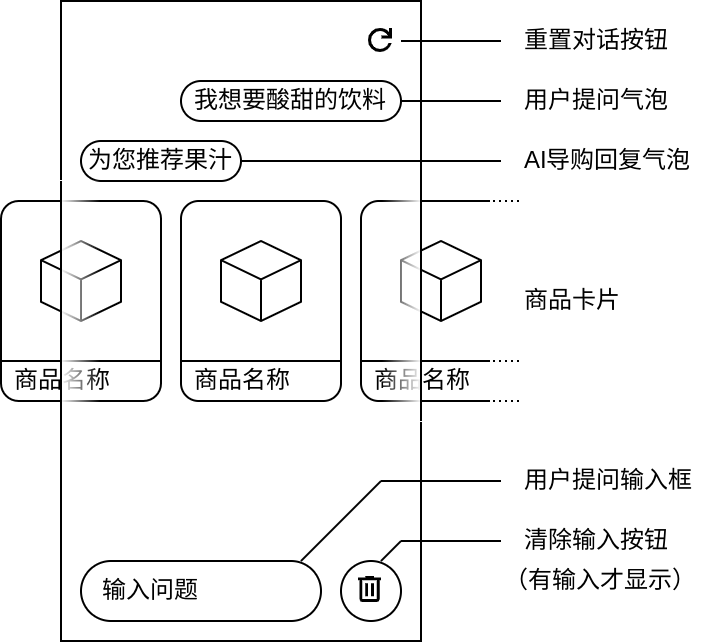
\includegraphics[width=0.8\textwidth, height=0.3\textheight, keepaspectratio]{./imgs/se-assist.png}
	\caption{最终消费者导购操作流程}
	\label{fig:se-assist}
\end{figure}

大模型输出的关键词被用于模糊搜索,搜索结果连同用户的原始输入和AI导购的答复将经过如图 \ref{fig:se-assist} 所示的用户界面展示给用户。值得注意的是,前文提及的使得大模型提取AI导购回答中搜索关键词的输入之中并无对输出(搜索关键词)格式的规定。这是因为将在后文提及的模糊搜索算法是为词组而不是句子优化的,对实际上搜索语句的格式并无要求,仅仅只需要语句中包含期望的关键词。即便大模型忽视了引导(“关键词”)而输出了相关的连贯句子,搜索步骤也可以正常进行。

\subsection{称重商品识别}

在许多类型的零售细分领域中,不可避免地将会遇到按重量计算,而本身并无包装(俗称“散装”)的产品,这些商品包括但不限于在生鲜蔬果、米面粮油和零食糖果等多种类别中的产品。实际上在社会上的许多商场和超市中,消费者在选购这些“散装”商品的时候,由自己完成的步骤只能持续至商品的挑拣和包装。最为重要的称重环节必须由店员帮助完成,并且因为明显地许多这些商品本身无法贴上条码或其他标签,店员需要在容器上粘贴同时记录了商品类型和质量的“静态标签”或与结算系统联网同步的“动态标签”。这种方式既有重复度较高、专业性较低的人工辅助参与,又需要非标准(EAN-13)的商品信息传递记录手段。

为了缓解这个问题,本设计的结算系统包含利用摄像头和AI图像识别技术的智能计重商品结算功能。

\subsubsection{数据准备}

\subsubsection{图像处理}

\subsubsection{AI图像分类}

\subsection{模糊搜索}

\subsubsection{商品数据处理}

\subsubsection{AI近义词搜寻}

\subsubsection{词典构建}

\subsubsection{搜索算法}